\chapter{Effets de taille finie}
    \label{chap-sos}
	
%%%%%%%%%%%%%%%%%%%%%%%%%%%%%%%
\section{Limite thermodynamique}
%%%%%%%%%%%%%%%%%%%%%%%%%%%%%%%

La fonction de partition d'un système dépend de la taille du système 
	
\begin{align}
    f_c(\beta,L,h) = - \frac{1}{L'} \frac{\delta \Omega(\beta,L,h)}{\delta L} \bigg|_{\beta,L'}
    \label{casimir-interface}
\end{align}

\begin{figure}
	\begin{minipage}[t]{0.5\linewidth}
		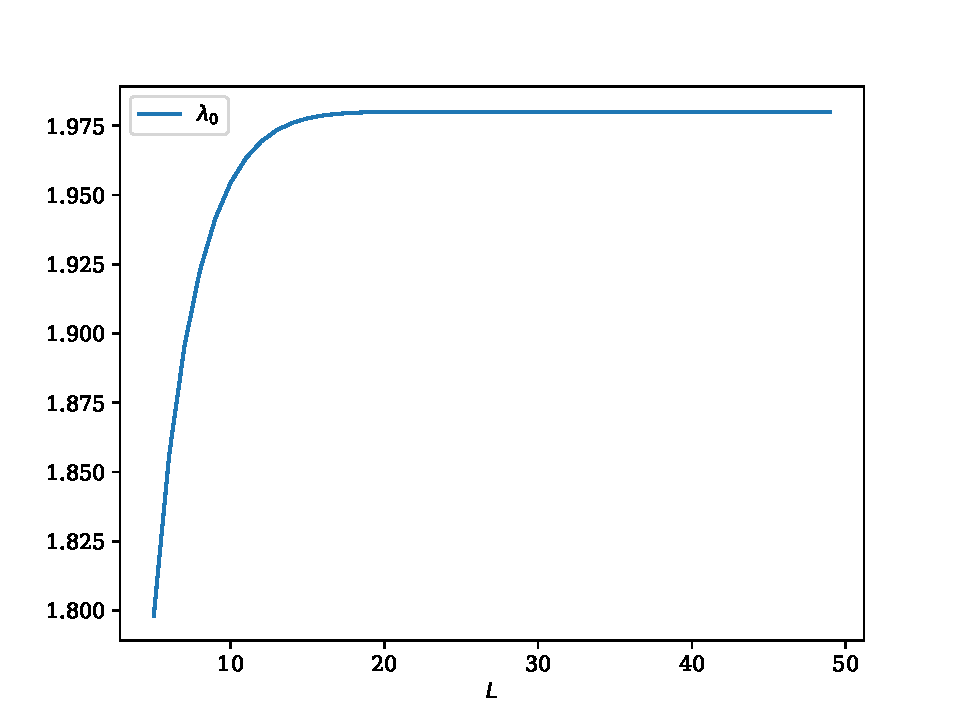
\includegraphics[width=\linewidth]{chap4/freeene-lambda0-mu.pdf}
	\end{minipage}%Cyclin
	\begin{minipage}[t]{0.5\linewidth}
		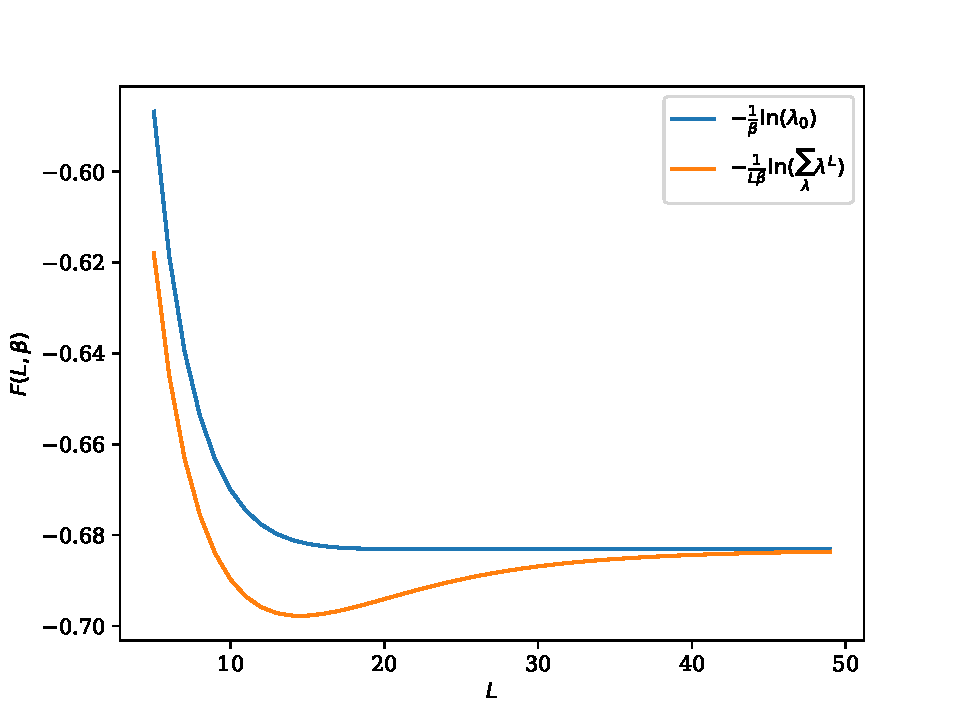
\includegraphics[width=\linewidth]{chap4/freeene-thermo-mu.pdf}
	\end{minipage}
	\caption{Plus grande valeur propre d'une interface libre en fonction de la taille $L$ du système pour $mu = 0.01$ et $\beta = 1$ (gauche)  ; énergie libre par site calculée via l'approximation de la limite thermodynamique \ref{energie-libre-site} comparé à la vraie fonction de partition \ref{partition-trace-lambda} en fonction de la taille $L$ du système pour $\mu=0.01$ et $\beta = 1$ (droite).}
	\vspace{-0.5cm}
\end{figure}  
	

\begin{figure}
    \centering
	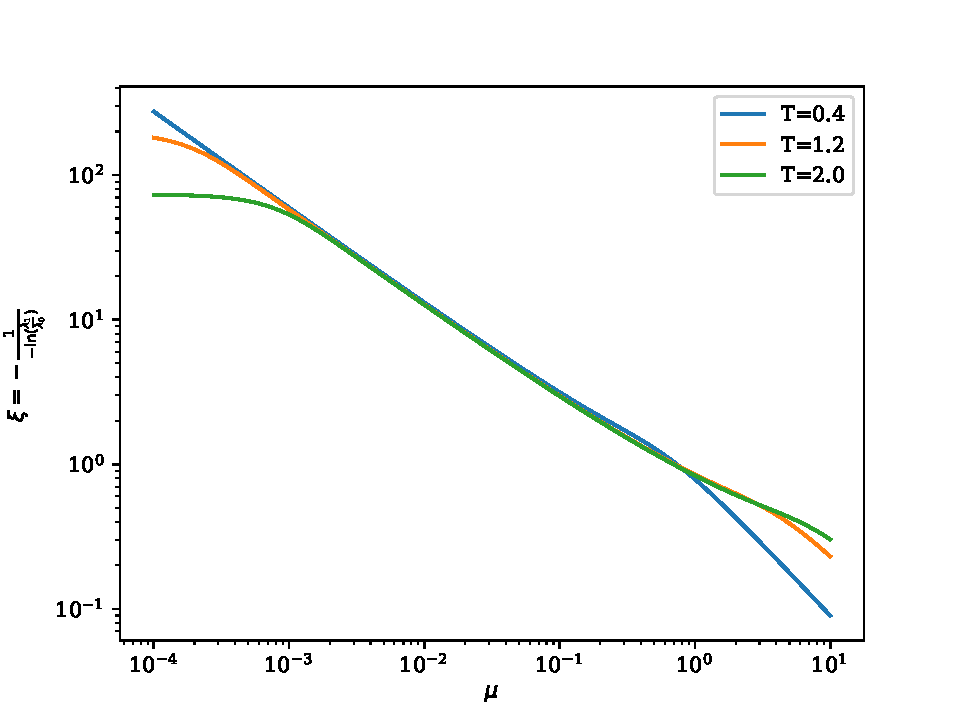
\includegraphics[width=0.5\linewidth]{chap4/longueur-correl.pdf}
    \caption{Longueur de corrélation à grande distance \ref{longueur-correl-thermo} pour une matrice $200\times200$ en fonction du potentiel chimique $\mu$ pour différentes températures.}
\end{figure}

\begin{figure}
    \centering
	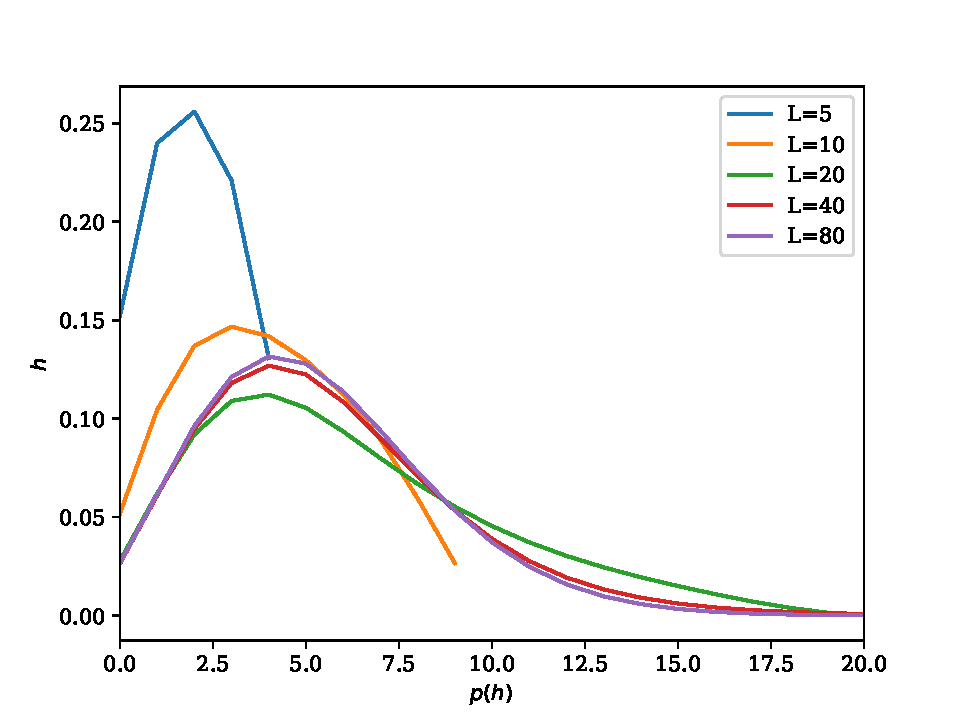
\includegraphics[width=0.5\linewidth]{chap4/distribution-taille-finie.pdf}
	\label{distribution-taille-finie}
	\caption{Distribution de l'interface pour différentes tailles de la matrice de transfert à $\mu=0.01$ et $\beta = 1$. Par un fit, la distribution ne suit pas une distribution de Poisson.}
\end{figure}


    \subsection{Paramètre d'ordre conservé}
	
    
    \subsection{Intégration sur le paramètre d'ordre}

%%%%%%%%%%%%%%%%%%%%%%%%%%%%%%%%%
    \section{Taille finie et effet Casimir critique}
    \label{sec-casimir}    
%%%%%%%%%%%%%%%%%%%%%%%%%%%%%%%%%

\begin{figure}
    \begin{minipage}[t]{0.5\linewidth}
        	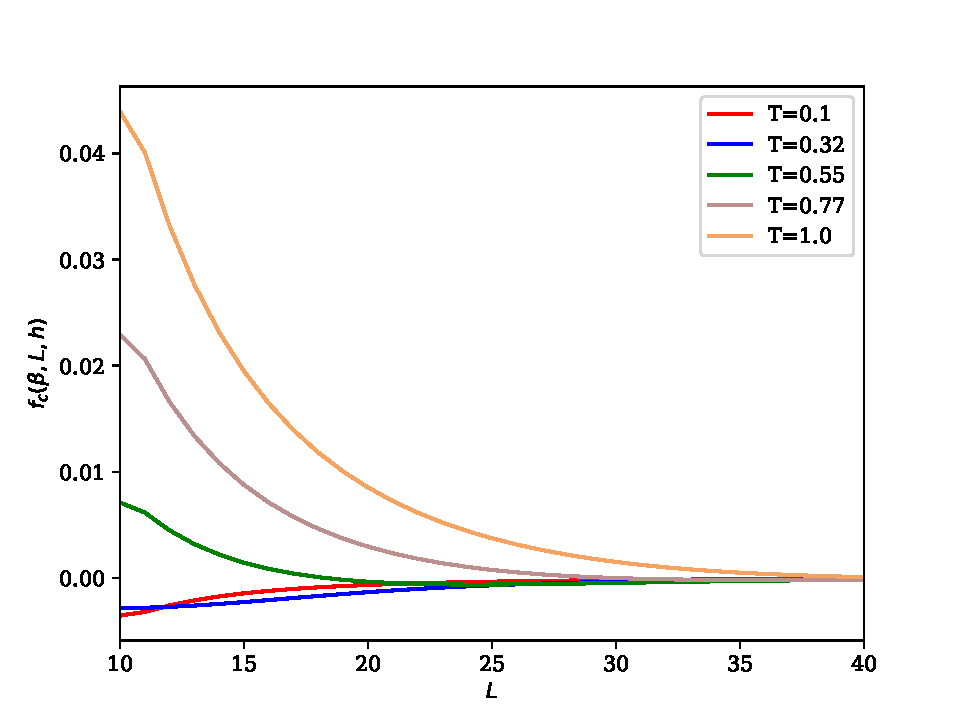
\includegraphics[width=\linewidth]{chap4/casimir-temperature.pdf}    
    \end{minipage}
    \begin{minipage}[t]{0.5\linewidth}
        	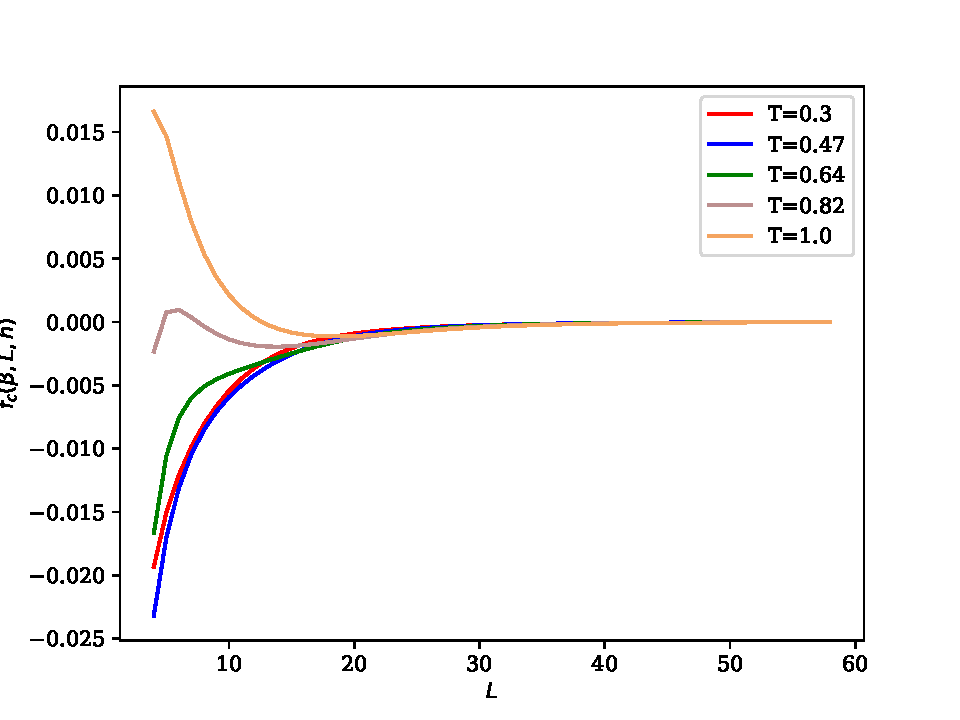
\includegraphics[width=\linewidth]{chap4/casimir-temperature-zoom.pdf}    
    \end{minipage}
	\label{distribution-taille-finie}
	\caption{Dérivée de l'énergie libre par rapport à la taille du système \ref{casimir-interface} pour différentes températures à $\mu=0.1$ (gauche) ; zoom sur la température seuil à $\mu=0.1$ comparé avec $\mu=0.05$ en pointillés (droite). }
\end{figure}


Dans la section \ref{sec-casimir} nous avons introduit l'effet Casimir comme étant le surplus d'énergie libre causé par le confinement du système, soit 
\begin{align}
    f_c(\beta,L,h) = - k_B T \frac{\partial(L \omega_{ex}(\beta,L,h))}{\partial L}\bigg|_{\beta,L'}
\end{align}
où $\omega_{ex}$ est l'énergie libre en excès dans le système, et prend une forme universelle proche du point critique \cite{casimir-universel}. Cet excès d'énergie libre est dûe à la frustration du système lorsque la longueur de corrélation est du même ordre de grandeur que la taille du système. Afin d'obtenir cette quantité dans les modèles sur réseau à partir de l'énergie libre totale, il est nécessaire de soustraire l'énergie du bulk au total. Néanmoins, dans les modèles d'interfaces qui nous intéressent, le seul terme extensif contribuant à l'énergie libre est l'énergie de surface, qui disparaît lorsque l'on prend la dérivée par rapport à la taille du système. Il n'est donc pas nécessaire de comparer l'énergie libre à la limite thermodynamique, et on obtient que 
 
    
    
Supposons un système 2D de taille $L \times L' $ où $L \less L'$. L'énergie libre $F(\beta,L,L') = - \frac{1}{\beta} \ln ( Z(\beta,L,L'))$ est une grandeur extensive lorsque la longueur de corrélation est plus petite que la taille du système $L$. 
Cette énergie libre peut se décomposer entre l'énergie de chaque phase par unité de volume $\omega_{bulk}$, et l'énergie de tension superficielle à l'interface par unité de surface $\omega_{surf}$ \cite{cardozo_finite_2015,lopes_cardozo_critical_2014}. À noter qu'à haute température dans un système complètement homogène, ce dernier terme disparaît.

Cependant, lorsque $\xi \simeq L$, la contrainte exercée sur les fluctuations thermiques par les conditions aux bords implique une modification de l'énergie libre, créant une force sur les parois. Cet effet, premièrement prédit par Hendrik Casimir\cite{h_b_g_casimir_attraction_1948}, fut étendu aux systèmes critiques\cite{nikolic_is_2017}, où la divergence de la longueur de corrélation rend les expériences bien plus faciles\cite{nguyen_controlling_2013}.

En présence d'un champ magnétique $h$ uniforme favorisant une phase par rapport à l'autre, l'énergie libre par unité d'aire d'un tel système se décompose \cite{lopes_cardozo_critical_2014,cardozo_finite_2015} en 
\begin{align}
    \frac{\Omega(\beta,L,L',h)}{L'} = L \omega_{bulk}(\beta,h) + \omega_{surf}(\beta,h) + L \omega_{ex}(\beta,L,h)
    \label{decomposition-energie}
\end{align}
où $\omega_{ex}(L,h)$ est le surplus d'énergie libre due au confinement des fluctuations, qui devient nul dans la limite $L\to \infty$.

La force de confinement par unité d'aire est définie par 
\begin{align}
    F_\perp(\beta,L,h) = - \frac{1}{L' }\frac{\partial \Omega(\beta,L,h)}{\partial L} \bigg|_{\beta,L'} = - k_B T \omega_{bulk}(\beta,h) - k_B T \frac{\partial(L \omega_{ex}(\beta,L,h))}{\partial L}\bigg|_{\beta,L'}
\end{align}
où le premier terme est la pression exercée par le système, tandis que le second terme est la force de Casimir par unité d'aire \cite{vasilyev_critical_2013} en $d$ dimensions 
\begin{align}
    f_c(\beta,L,h) = - k_B T \frac{\partial(L \omega_{ex}(\beta,L,h))}{\partial L}\bigg|_{\beta,L'} = k_B T L^{-d} \Theta(u_t,u_h)
    \label{casimir-scaling}
\end{align}
où $u_T = \frac{T-T_C}{T_C} L^\frac{1}{\nu}$ et $u_h = \frac{h}{k_B T_C} L^\frac{\beta+\gamma}{\nu}$ et où les exposants $\beta$, $\gamma$ et $\nu$ sont des exposants universels reliés aux amplitudes universelles des longueurs de corrélation du système \cite{pelissetto_critical_2002,vasilyev_critical_2013} et $\Theta(u_t,u_h)$ est une fonction universelle propre à chaque modèle. Cette fonction universelle dépend des conditions aux bords du système \cite{dantchev_casimir_2017,dantchev_exact_2016} ainsi que de l'ensemble thermodynamique dans lequel on se place \cite{gross_critical_2016,rohwer_transient_2017}.

Afin d'extraire la force de Casimir, il suffit alors de soustraire deux quantités extensives, c'est-à-dire en utilisant deux largeurs différentes $L_1$ et $L_2$
\begin{align}
    f_c(\beta,L_1,h) - f_c(\beta,L_2,h) =  \frac{1}{L' }\frac{\partial \Omega(\beta,L_2,h)}{\partial L} \bigg|_{\beta,L'} -  \frac{1}{L' }\frac{\partial \Omega(\beta,L_1,h)}{\partial L} \bigg|_{\beta,L'}
\end{align}
Puisque le surplus d'énergie dû au confinement est nul lorsque $L_2\to \infty$, on obtient que la force de Casimir est
\begin{align}
    f_c(\beta,L_1,h) \simeq \frac{1}{L' }\frac{\partial \Omega(\beta,L_2,h)}{\partial L} \bigg|_{\beta,L'} -  \frac{1}{L' }\frac{\partial \Omega(\beta,L_1,h)}{\partial L} \bigg|_{\beta,L'}
    \label{casimir-diff-omega}   
\end{align}
où en utilisant \ref{casimir-scaling}, l'approximation est valable dans le cas où $ \left( \frac{L_2}{L_1}\right)^{-d} \ll 1 $.  Cette force étant une force émergente d'origine entropique, la somme des forces exercées individuellement par chaque particule du système n'est pas égale à la force totale appliquée sur le système\cite{paladugu_nonadditivity_2016}.

La détection expérimentale de ce phénomène se fait traditionnellement dans des fluides binaires par \textit{Total Internal Reflection Microscopy} (TIRM) \cite{fukuto_critical_2005,hertlein_direct_2008,gambassi_critical_2009,edison_critical_2015-1}. La méthode consiste à mesurer le potentiel d'une sphère flottant sur un fluide binaire critique reposant sur une plaque. Cette sphère et cette plaque sont traitées chimiquement afin de favoriser l'une des deux phases à leu voisinage. Ainsi il est possible de créer des conditions aux bords $(++)$, $(+-)$ ou $(--)$ qui modifient la forme de la fonction universelle \ref{casimir-scaling}. À l'inverse, il est possible de mesurer la force de Casimir \cite{nguyen_controlling_2013} afin d'étudier les transitions de phases colloïdales.

Le modèle d'Ising appartient à une classe de modèles où il est facilitant l'obtention de résultat analytique \cite{hobrecht_critical_2017} comparables aux simulations numériques \cite{vasilyev_monte_2007,vasilyev_universal_2009,cardozo_finite_2015}.

Jusqu'à présent nous avons parlé de systèmes à l'équilibre, mais l'effet des fluctuations est également présent en dehors de l'équilibre. L'étude des interfaces nous mène à proposer des modèles de cisaillement qui influencent les propriétés statistiques des systèmes, et ainsi modifier la force de Casimir \cite{dean_out--equilibrium_2010}.


%%%%%%%%%%%%%%%%%%%%%%%%%%%%%%%%%%
\section{Hamiltonien de transition}
\label{sec-transition}
%%%%%%%%%%%%%%%%%%%%%%%%%%%%%%%%%%

Nous avions vu à l'équation \ref{casimir-diff-omega} que la force de Casimir par unité d'aire se calcule à partir de la variation de l'énergie libre $\Omega$
\begin{align}
    f_c(\beta,L_1,h) \simeq \frac{1}{L' }\frac{\partial \Omega(\beta,L_2,h)}{\partial L} \bigg|_{\beta,L'} -  \frac{1}{L' }\frac{\partial \Omega(\beta,L_1,h)}{\partial L} \bigg|_{\beta,L'}
\end{align}

En suivant \cite{vasilyev_monte_2007,cardozo_finite_2015} pour un système d'Ising carré de taille $L \times L'$, l'idée est de calculer la dérivée continue par rapport à une taille discrète du système $L$ en interpolant le système via l'Hamiltonien de transition
\begin{align}
    \mH_{tr}(\lambda) = (1-\lambda) \mH_0 + \lambda \mH_1
    \label{hamil-trans}
\end{align}
où $\mH_0$ est l'Hamiltonien d'un système de hauteur maximale $L$, et $\mH_1$ l'Hamiltonien d'un système de hauteur maximale $L-1$ où on a découplé une couche (voir Figure \ref{decouplage}). L'énergie libre associée à cet Hamiltonien est
\begin{align}
    \Omega_{tr}(\lambda) = -k_B T \ln \left( \sum_{h_1 ... h_L} e^{-\beta \mH_{tr}(\lambda)} \right)
\end{align}
De la dérivée de l'énerie libre découle
\begin{align}
    \frac{\Omega_{tr}(\lambda)}{d\lambda} = < \mH_1 - \mH_0>_{\mH_{tr}(\lambda)}
\end{align}
où $< · >_{\mH_{tr}(\lambda)}$ représente la moyenne statistique sur le système en transition, facilement calculable dans les simulations numériques. En intégrant sur le couplage, on trouve au final que
\begin{align}
    \Omega_1 - \Omega_0 = \int_0^1 d\lambda  < \mH_1 - \mH_0>_{\mH_{tr}(\lambda)}
\end{align}
Finalement, dans la limite où l'épaisseur du système est suffisement grande pour que la variation d'une couche soit suffisement petite ($L' \gg 1$), on trouve que
\begin{align}
   - \frac{\partial \Omega(\beta,L,h)}{\partial L} \bigg|_{\beta,L'} \simeq  \int_0^1 d\lambda  < \mH_1 - \mH_0>_{\mH_{tr}(\lambda)}
\end{align}

\begin{figure}
	\begin{minipage}[t]{0.3\linewidth}
		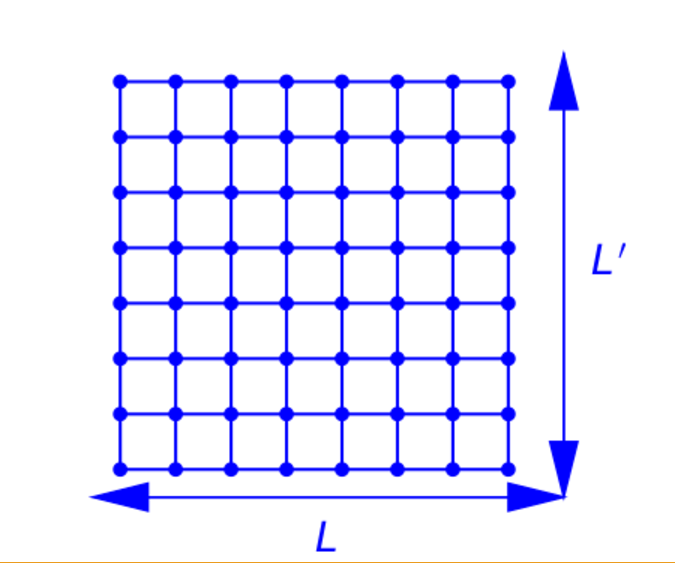
\includegraphics[width=\linewidth]{numerical/cross-h0.pdf}
		\caption*{$\mH_0$}
	\end{minipage}
	\begin{minipage}[t]{0.3\linewidth}
		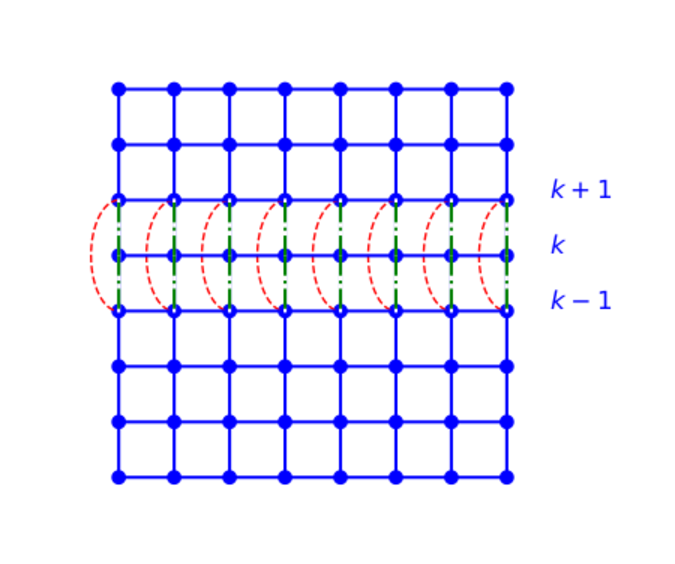
\includegraphics[width=\linewidth]{numerical/cross-hlambda.pdf}
		\caption*{$\mH(\lambda)$}		
	\end{minipage}
	\centering
	\begin{minipage}[t]{0.3\linewidth}
		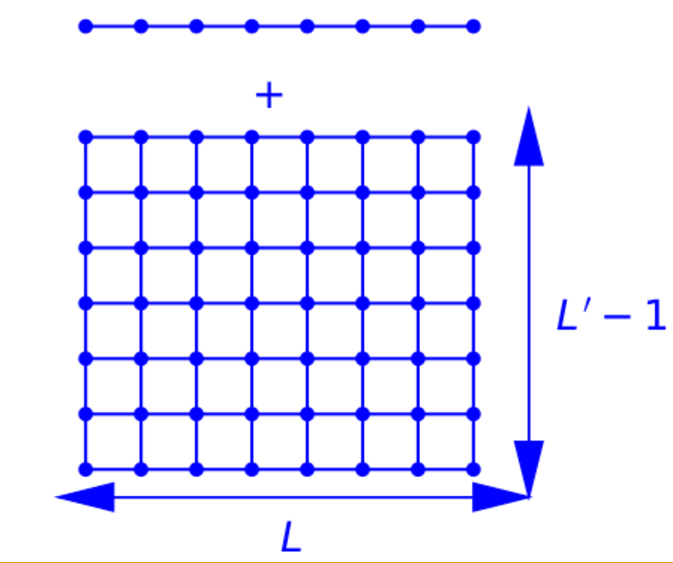
\includegraphics[width=\linewidth]{numerical/cross-h1.pdf}
		\caption*{$\mH_1$}
	\end{minipage}
	\caption{Découplage progressif de la $k$-ième couche du système afin de calculer la variation de l'énergie libre grâce à l'hamiltonien de transition. Les liens en bleu ont une énergie de $\beta J$, les liens en rouge une énergie de $\lambda \beta J $ et les liens en vert une énergie de $ (1-\lambda) \beta J$. Reproduction 2D de \cite{vasilyev_monte_2007}.}
	\label{decouplage}
\end{figure}

Pour le modèle Solid-On-Solid, il est possible de calculer la variation d'énergie créée par le découplage directement. Si le découplage s'est créé à la rangée $k$, on ajoute un lien d'énergie $\lambda J$ entre les rangées $k-1$ et $k+1$ et on retire $\lambda J$ énergie des rangées $k-1$ à $k$  et de $k$ à $k+1$. On obtient
\begin{align}
    &\mH_{tr,SOS}(\lambda) = \mH_{0,SOS} - \nn
     &\frac{\lambda J}{2} \sum_x \left[ \sgn(k-1-h(x)) \sgn(k+1-h(x)) - \sgn(k-h(x)) \left( \sgn(k-1-h(x))+\sgn(k+1-h(x)) \right) \right]
\end{align}
où le facteur $\frac{1}{2}$ est obtenu afin de prendre en compte le coefficient $2$ dans \ref{energie-sos-ising}.

\begin{figure}
    \centering
	\includegraphics[width=0.5\linewidth]{example-image-a}
	\caption{Effet Casimir pour Glauber avec TM, hamiltonien de transition et intégation magnétique, pour Kawasaki avec Hamiltonien de transition}
\end{figure}
	
	
	\section{Effet du cisaillement}


\begin{figure}
    \centering
	\includegraphics[width=0.5\linewidth]{example-image-b}
	\caption{Effet Casimir pour Kawasaki avec cisaillement pour différent $\mu$}
\end{figure}

%%%%%%%%%%%%%%%%%%%%%%%%%%%%%%%
    \section{Conclusion}
%%%%%%%%%%%%%%%%%%%%%%%%%%%%%%%	
	
	Il existe par ailleurs de nombreuses sources contribuant à l'énergie totale du système : l'énergie du volume (\textit{bulk}) du système, l'énergie de l'interface définie par sa tension superficielle \ref{tension-superficielle}, et une énergie d'excès qui donne naissance à la force de Casimir \ref{casimir-scaling}. Cette force est dûe au confinement du système par des conditions aux bords contraignant les fluctuations du champ $\phi$ selon une direction. 
Nous avons également vu une manière d'obtenir la fonction universelle de la force de Casimir critique via le découplage progressif d'une couche du système, afin que dans la limite où $L' \gg 1$, ce découplage s'apparent à la dérivée discrète de l'énergie libre (section \ref{sec-transition}). Dans le chapitre \ref{chap-sos}, nous étudions une manière moins générale d'obtenir cette énergie libre par de l'intégration d'une autre vari
